\section{Desarrollo de la librería}

La librería es nombrada como \textbf{L.A.M.F.R.I.A} que significa: Librería para el análisis de multifractalidad y robustez con algoritmos de inteligencia artificial.

\subsection{Procesamiento de redes con SNAP}

Este trabajo es desarrollado con el apoyo de la librería SNAP de la Universidad de Standford \url{https://snap.stanford.edu}, la cual está escrita en C++ y se encuentra optimizada para redes de gran tamaño, gracias al uso de una representación basada en matrices dispersas.

Para la implementación de los algoritmos se utiliza el lenguaje de Programación Python y el entorno que ofrece esta librería para este lenguaje. La elección del lenguaje se debe a que actualmente es tendencia para el desarrollo de aplicaciones Inteligencia Artificial, el cual es el enfoque de este proyecto. Esto permite a futuro los algoritmos utilizados puedan ser integradas con mayor facilidad con otras estrategias de inteligencia artificial.

\subsubsection{Selección de SNAP frente a otras librerías}

En el mercado se destacan algunas librerías para el procesamiento de redes complejas como:

\begin{itemize}
    \item NetworkX: Es una librería de Python comúnmente utilizadas, pero no es recomendada con redes de más de 100000 nodos
    \item IGraph: Utilizada en Python y R, está enfocada a estudio de propiedades y representación gráfica que a procesamiento de redes de gran tamaño.
    \item sigma.js, escrita en JavaScript, sin embargo, el lenguaje no es recomendado para procesamiento si no para visualización.
\end{itemize}

La selección de SNAP se debe a lo siguiente:

\begin{enumerate}
    \item Está escrita en C++, lo que permite a la librería administrar directamente la memoria.
    \item En Python se utiliza una interfaz a las funciones escritas en C++, por lo que el código se ejecuta directamente en la máquina, evitando el paso por el interpretador del lenguaje.
    \item Se utilizan matrices dispersas para la representación de las redes, lo que permite reducir la complejidad computacional de operaciones y reducir el espacio requerido en memoria.
    \item La librería está diseñada para el procesamiento de redes a gran escala y ha sido ampliamente probada en diferentes problemas y escenarios.
    \item Se cuenta con un gran documentación y un foro en el cual la comunidad de desarrolladores da solución a problemas que se puedan presentar.
    \item Es una librería independiente, lo que permite exportarla fácilmente a diferentes entornos computacionales.
\end{enumerate}


\subsection{Arquitectura de la librería}

La librería desarrollada es un conjunto de funciones que corren sobre SNAP. En la figura \ref{fig:diagramaConceptual} se provee un diagrama conceptual de la librería.

\begin{figure}[H]
    \centering
    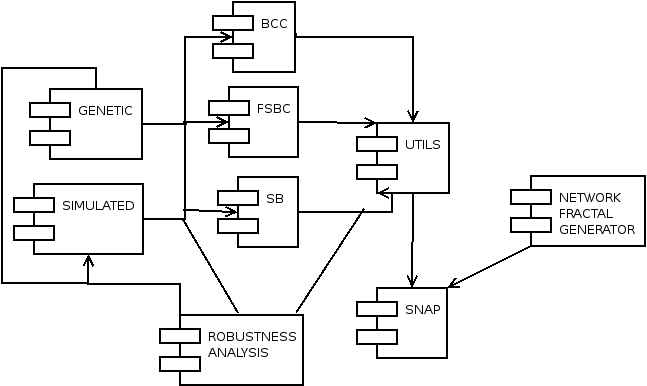
\includegraphics[scale=0.7]{Capitulo7Libreria/imagenes/componentes.png}
    \caption{Diagrama conceptual de L.A.M.F.R.I.A}
    \label{fig:diagramaConceptual}
\end{figure}

\begin{itemize}
    \item SNAP: Provee las funciones de carga y búsqueda en redes complejas
    \item UTILS: Provee funciones generales para los algoritmos, como es el caso de cálculo de matrices de adyacencia o conectividad. Así mismo funciones para la carga y guardado de archivos
    \item BCC: Algoritmo de Box Compact Counting
    \item FSBC: Algoritmo de Fixed Size Box Counting
    \item DB: Algoritmo de SandBox
    \item Network Fractal Generator: Ofrece funciones para la creación de (2,2)-flower y (1,3)-flower de cualquier generación
    \item Genetic y Simulated ofrecen las estrategias de IA. Estas hacen parte de la ejecución de los algoritmos ya que calculan los centros de cajas y se ejecuta el algoritmo con esta configuración
    \item Robustness Analysis: Realiza el análisis de robustez, permite utilizar todos los algoritmos para el análisis de multifractalidad a medida que se pierden nodos. En las pruebas solo se usó el algoritmo SandBox por cuestiones de tiempo.
\end{itemize}